\documentclass{article}
\usepackage{importer}
\usepackage[backend=biber]{biblatex}
\addbibresource{kilder.bib}

\title{Faste Stoffers Fysikk: Løsningsforslag til øvinger}
\author{Sebastian Siljuholtet Johansen}
\date{Vår 2024}

\begin{document}

\maketitle

\newpage
\section*{Ingress}
Skrevet av studenter. Notater er tatt under forelesningene i TFY4220 Faste Stoffers Fysikk av Dag Werner Breiby og er veldig basert på boken Introduction to Solid State Physics av C. Kittel. Øvingene er løst av Sebastian Siljuholtet Johansen.

\newpage
\tableofcontents

\newpage
\oving{1}
\oppgave{1}
\deloppgave{a}
Hva er den mattematiske definisjonen til en krystall? Vel, man kan definere en krystall som et periodisk gitter med ulike symmetrier knyttet til ethvert krystall. Krystallene er videre bygget opp av en basis knyttet til hvert gitter som er knyttet til hvilke atomer som er plassert hvor og koblet til hvilke andre atomer. Matematisk blir da krystallen konvolusjonen av gitteret med basisen.

Altså blir en krystall en periodisk struktur av bygningsblokker. Disse bygningsblokkene kan være atomer, parr med atomer, komplekse molekyler eller liknende.

Vi skriver mattematisk derfor fra over at:
\begin{equation}
    C(x) = \underbrace{G(x)}_{\text{gitterstrukturen}}\otimes \underbrace{B(x)}_{\text{basisen}}
\end{equation}
\deloppgave{b}
Et primitivt gitter i tre dimensjoner er definert av tre vektorer $\vec{a}_1, \vec{a}_2$ og $\vec{a}_3$ slik at enhver vektor mellom gitterpunkt $\Vec{T}$ kan bli beskrevet som:
\begin{equation}
    \vec{T} = u_1 \vec{a}_1+ u_2 \Vec{a}_2 +  u_3 \Vec{a}_3
\end{equation}
hvor $u_1, u_2$ og $u_3$ er vilkårlige heltall. 
\deloppgave{c}
Den primitive Wigner-Seitz-cellen er definert gjennom å lage linjer mellom alle de nærmest gitterpunktene og deretter lage tversgående plan halvveis på midten av alle disse. Det minste volumet som skapes av disse planene er da Wigner-Seitz-cellen.
\deloppgave{d}
En trefoldig rotasjon er en rotasjon på 120 grader. En n-foldig rotasjon er en rotasjon på $\frac{360}{n}$ grader. Hvis noe er invariant under en slik rotasjon vil den være lik på 
\oppgave{2}
\deloppgave{a}
Bikakegitteret er ikke et primitivt gitter fordi det finnes to forskjellige typer punkter i det. Altså har vi ikke bare samme type gitterpunkt. Derfor må bikakegitteret bestå av en basis av to atomer og et primitivt gitter i bakgrunnen. En illustrasjon av de ulike typene er de blå og rød atomene her:
\begin{figure}[H]
    \centering
    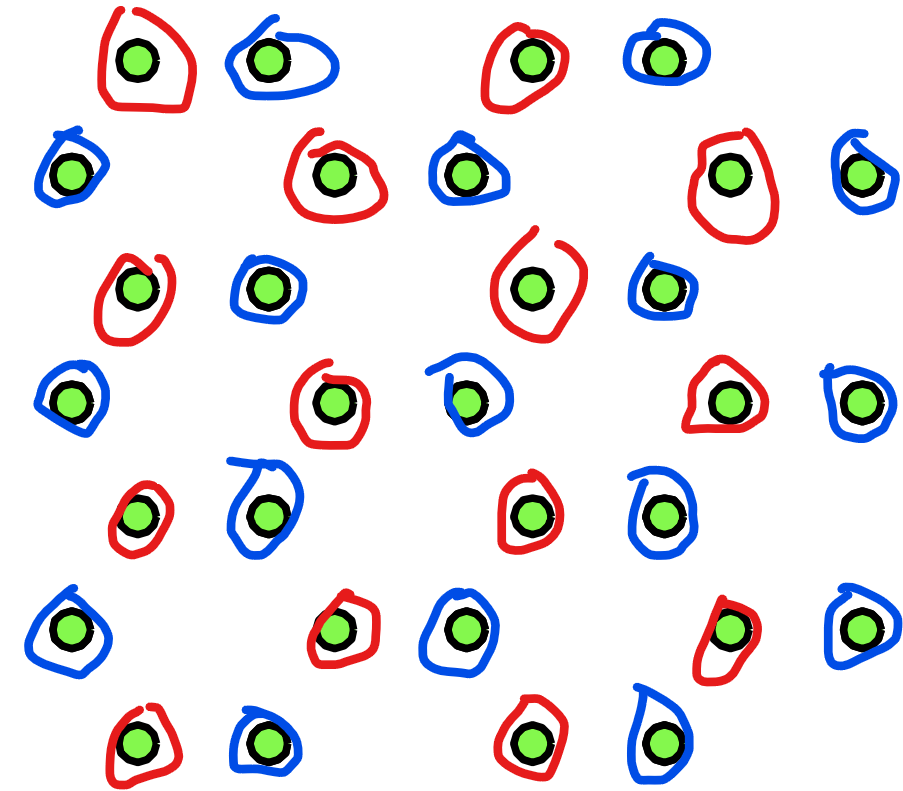
\includegraphics[width=0.2\linewidth]{bilder_lf/bikake_gitterstruktur.png}
    \caption{Strukturen i bikakegitteret}
    \label{fig:bikake_gitterstruktur}
\end{figure}
Her må basisen bestå av et rødt og et blått atom. Videre må det primitive gitteret bestå av kun en av fargene. Dette Bravaisgitteret må være et skrått rektangulært mønster.
\deloppgave{b}
Et Bravais-gitter kan bli beskrevet på to måter:
\begin{itemize}
    \item En uendelig mengde med diskré punkter som er arrangert på en måte som ser likt ut uansett hvor du er og hvordan orientasjonen er.
    \item Alle punkter som er beskrevet på formen: $\vec{R}_{mno} = m \vec{a} + n\vec{b} + o\vec{c}$ hvor $m, n$ og $o$ er heltall og vektorene er vilkårlige. Her må også vektorene være lineært uavhengige og dermed ikke i samme plan eller linje. 
\end{itemize}
\deloppgave{c}
Flere forskjellige typer enhetsceller vi kan velge her er de som er i bildet under:
\begin{figure}[H]
    \centering
    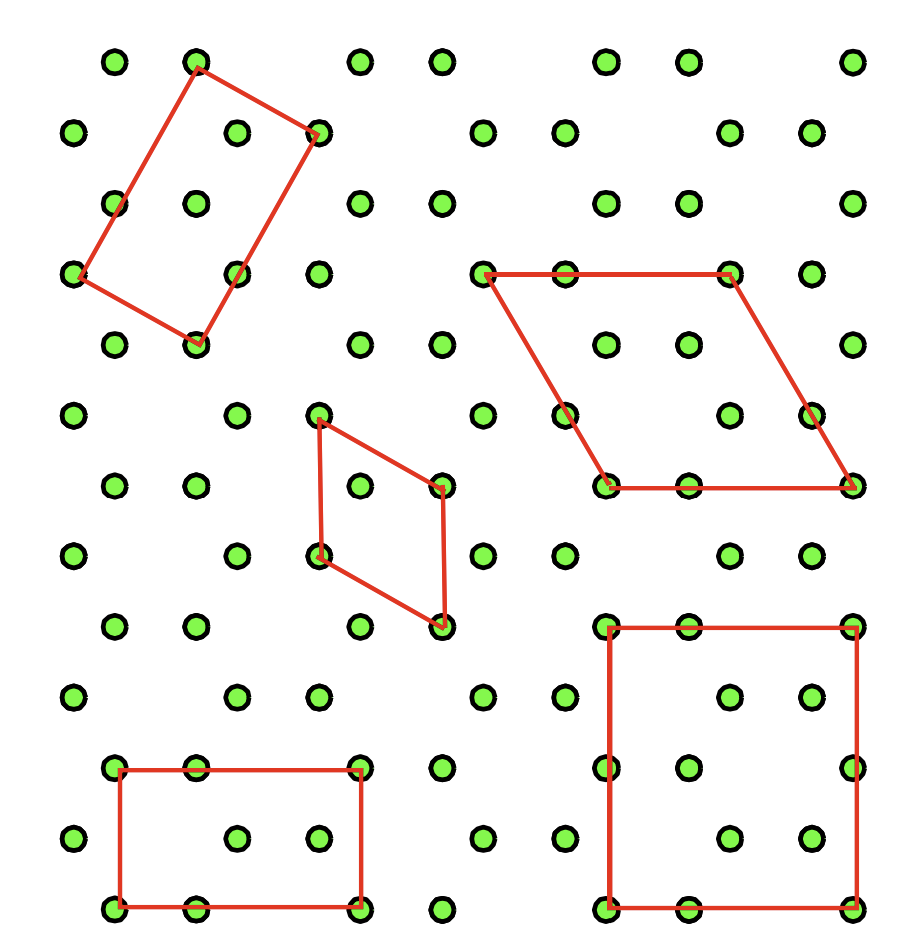
\includegraphics[width=0.25\linewidth]{bilder_lf/typer_enhetsceller_i_bikakegitteret.png}
    \label{fig:typer_enhetsceller_i_bikakegitteret}
    \caption{Noen enhetsceller i bikakegitteret}
\end{figure}
Den mest normale typen enhetscelle er den definert på måten beskrevet i deloppgave a). Her har vi at strukturen blir heksagonal med to atomer i basisen hvor vinkelen mellom vektorene som beskriver Bravais-gitteret blir 120 grader. Dette blir da enten det røde eller det røde gitteret i figuren fra deloppgave a) (\ref{fig:bikake_gitterstruktur})
\oppgave{3}
\deloppgave{a}
\begin{enumerate}
    \item For en romsentrert kubisk (B.C.C) struktur med sfærer, vil vi få en sfære på hvert gitterpunkt. ALtså en kube med sfærer på hvert hjørne og en i midten. Vi antar at kuben har sidekanter med lengde 1. Da må sfærene ha radius 0.5. Derimot gjør sfæren i midten at vi må ha en radius som tilsvarer at 4 radiuser (en fra to hjørner og to fra midten) går over diagonalen som får lengde $\sqrt{3}$. Altså blir radiusen til sfærene $\frac{\sqrt{3}}{4} = \frac{1}{2 \sqrt{2}}$. Volumet til disse sfærene vil bli det samme som 8 sfærer med bare en åttendedel fra hver og hele den i midten. Altså totalt to sfærer med den radiusen. De får volum: $V = 2 * 4 \pi \left(\frac{\sqrt{3}}{4}\right)^3 / 3 = \frac{\pi \sqrt{3} 3}{24} = 0.68017476158$. Altså blir pakkeprosenten på $68.0174\%$
    \item For en FCC-pakket sfære må vi først se på sidene. Her får vi 9 sfærer som vi kan identifisere på hver side. Dette vil gi oss at den aller høyeste radiusen vi kan få på sideflatene er $1/4$ av diagonalen på en flate. Altså $\sqrt{2} / 4$. siden vi kan ha 4 radiusen totalt over en sideflate. Da vil vi få 1 sfære siden vi ikke har noen i midten nå. Sideflatene gir oss 3 sfærer til. Altså får vi et totalt volum: $V = 4 * 4 * \pi \left(\frac{\sqrt{2}}{4}\right)^3 / 3 = 2 \sqrt{2} \pi / 12 = 0.74048048969$ som gir oss en pakkeprosent på $74.048\%$.
\end{enumerate}
\deloppgave{b}
Forholdet her blir:
\begin{align}
    \frac{\Phi_{f.c.c}}{\Phi_{b.c.c}}\frac{\frac{\pi \sqrt{3} 3}{24}}{2 \sqrt{2} \pi / 12} = \frac{3}{4} \sqrt{\frac{3}{2}} = 0.91855865354
\end{align}
\oppgave{4}
\deloppgave{a}
\begin{enumerate}
    \item Her vil vi få indeksene $(hkl) = (\bar{1}21)$ siden forholdene er inversen av disse.
    \item Her vil få få indeksene $(hkl) = (0\bar{2}0)$ siden $1/|a_1| = 1/|a_3| = 1 / \infty$, mens $1 / |a_2| = 1 / (- 1/2) = -2$.
\end{enumerate}
\deloppgave{b}
Et generelt plan med (hkl) indekser kan bli tegnet på følgende måte (\ref{fig:hkl_plan}):
\begin{figure}[H]
    \centering
    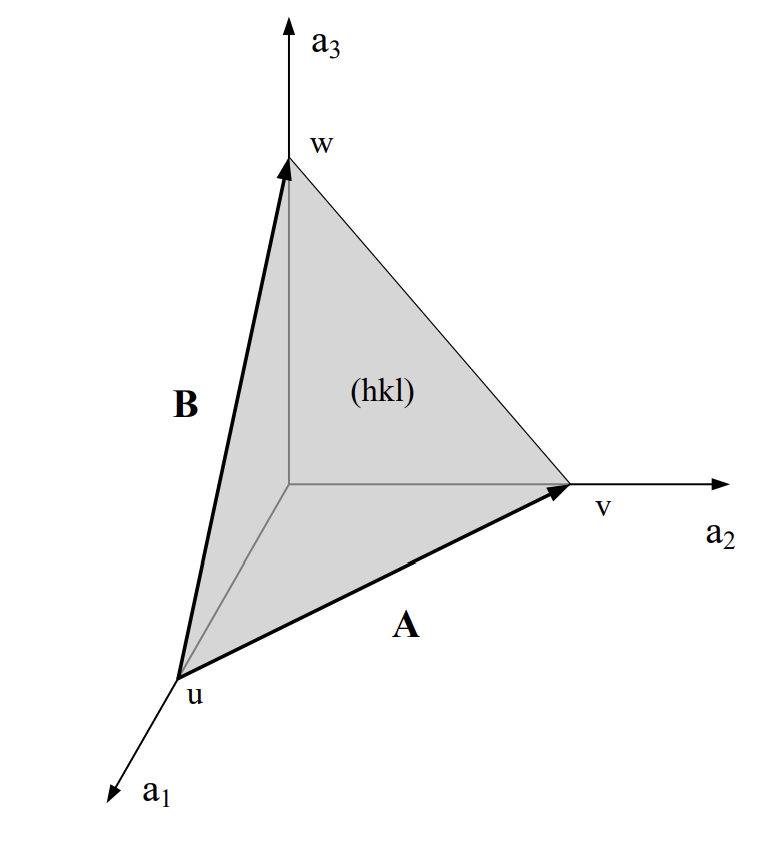
\includegraphics[width=0.5\linewidth]{bilder_lf/hkl_plan.png}
    \caption{Generelt (hkl) plan}
    \label{fig:hkl_plan}
\end{figure}
Her kan vektorene A og B spenne planet. Disse er definert som:
\begin{align}
    \vec{A} = -u \vec{a}_1 + v\vec{a_2}\\
    \vec{B} = -u \vec{a}_1 + w\vec{a_3}
\end{align}
Normalvektoren til dette planet er kryssproduktet til disse vektorene. Dette blir som følger:
\begin{align}
    \vec{A} \times \vec{B} = uvw( \frac{1}{u} \vec{a}_1+\frac{1}{v} \vec{a}_2+\frac{1}{w} \vec{a}_3)
\end{align}
Inversen av disse lengdene er jo $hkl$ lengdene våre multiplisert med en konstant. Altså har vi at:
\begin{align}
    \vec{A} \times \vec{B} &= uvw( \frac{1}{u} \vec{a}_1+\frac{1}{v} \vec{a}_2+\frac{1}{w} \vec{a}_3) \\
    &= uvw( Kh \vec{a}_1+Kk \vec{a}_2+Kl \vec{a}_3)\\
    &= uvw K\underbrace{( h \vec{a}_1+k \vec{a}_2+l \vec{a}_3)}
\end{align}
Og dermed ser vi at vektoren som har parantes under seg. Denne vektoren er jo vektoren i retningen (hkl). Altså må planet i seg selv være ortogonalt med denne vektoren siden planets normalvektor er parallelt med den retningen.
\deloppgave{c}
Den normaliserte normalvektoren vår i dette tilfellet blir:
\begin{equation}
    \vec{n}= \frac{ \vec{A} \times \vec{B}}{| \vec{A} \times \vec{B}|} = \frac{1}{a} \frac{( h \vec{a}_1+k \vec{a}_2+l \vec{a}_3)}{\sqrt{h^2 + k^2 + l^2}}
\end{equation}
Planene vil bli en forskyvning langs aksene med en lengde 1. Altså vil vi finne lengden mellom planene til å være en translasjon langs en av aksene prosjektert på  normalvektoren. Da vil få få:
\begin{align}
    d_{hkl} &= \frac{\vec{a}_i \cdot \vec{n}}{(h, k, l)} \\
    &= \frac{1}{(h, k, l)} \frac{(h, k, l) |\vec{a}_i|^2}{a \sqrt{h^2 + k^2 + l^2}} \\
    &= \frac{a^2}{a\sqrt{h^2 + k^2 + l^2}} \\
    &= \frac{a}{\sqrt{h^2 + k^2 + l^2}}
\end{align}
\deloppgave{d}
Tettpakningen i FCC krever følgende bilde:
\begin{figure}[H]
    \centering
    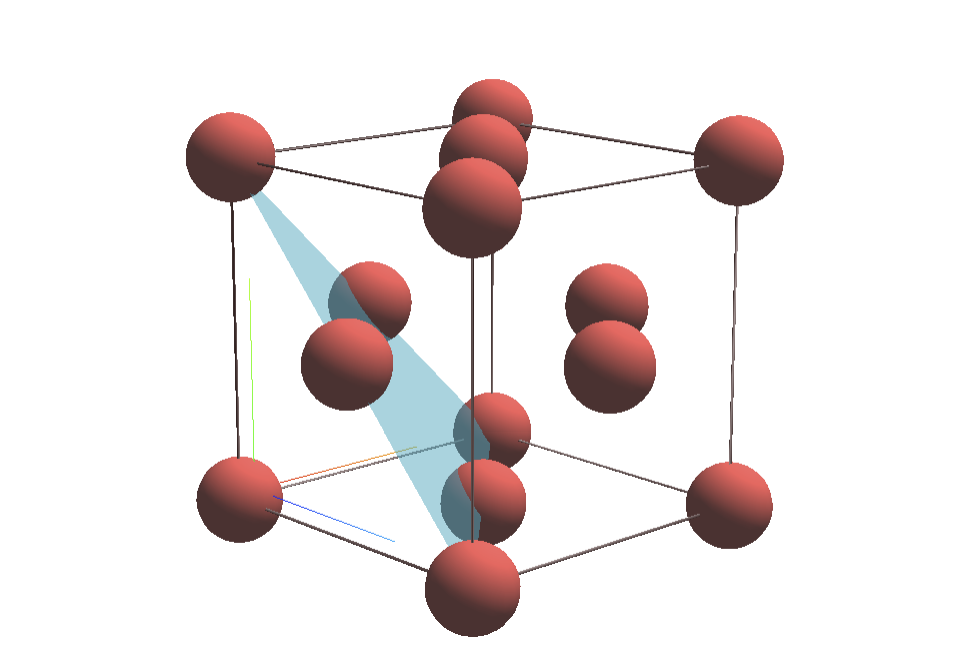
\includegraphics[width=0.5\linewidth]{bilder_lf/tettpakning_fcc.png}
    \caption{Plan FCC}
    \label{fig:tettpakning_fcc}
\end{figure}
Her har vi ikke tegnet et tettpakket gitter, men man kan se hvilket plan som må til for å få FCC-gitteret. Dette planet er da (111) planet.
På samme måte kan vi se hvilket plan som må til for BCC gitteret. Her blir det igjen noe tegnet som:
\begin{figure}[H]
    \centering
    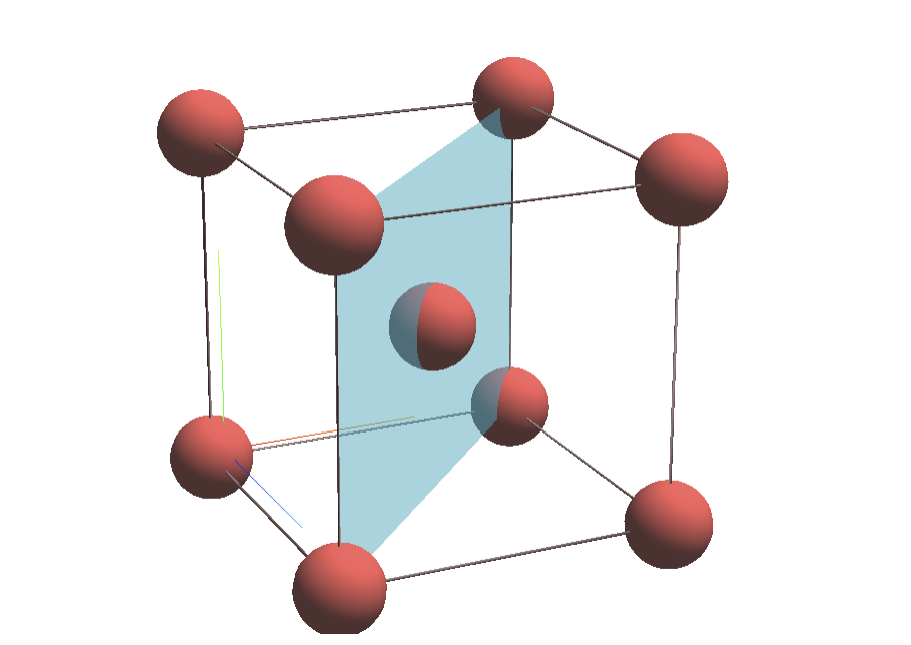
\includegraphics[width=0.5\linewidth]{bilder_lf/tettpakket_bcc.png}
    \caption{Plan BCC}
    \label{tettpakket_bcc}
\end{figure}
som gir oss planet (110).

I begge bildene over er origo nederst til venstre.
\nyside
\oving{2}
\oppgave{1}
\deloppgave{a}
Periodisiteten til elektronenes tetthet i et gitter må være likt som gitteret. Derimot gjelder ikke dette bare tettheten deres men også alle andre lokale egenskaper.
\deloppgave{b}
Mattematisk skriver man relasjonen slik:
\begin{equation}
    e^{i \vec{G} \cdot \vec{r}} = 1
\end{equation}
hvor $\vec{G}$ er en resiprokalvektor og hvor $\vec{r}$ er en normal vektor. Mattematisk er resiprokalgitteret fouriertransformen av det normale gitteret.
\deloppgave{c}
En bølgevektor $\vec{k}$ lever i resiprokalgitteret og beskriver en forplantene bølge med momentum $\vec{p} = \hbar \vec{k}$ og med bølgelengde $\lambda = \frac{2\pi}{|\vec{k}|}$
\deloppgave{d}
Wigner-Seitz cellen er den første brillouinsonen i resiprokalgitteret. Egentlig sier man dette motsatt vei, med at Resiprokalgitteres Wigner-Seitz celle er den første brillouinsonen.
\deloppgave{e}
En lengde $L$ vil bli til $\frac{2\pi}{L}$ i resiprokalgitteret. Altså har vi:
\begin{equation}
    V = L^3 \Rightarrow \frac{(2\pi)^3}{L^3} = \frac{(2\pi)^3}{V} = V^*
\end{equation}
Dette gjelder derimot bare for kvadratiske celler. Altså må vi generelt gjøre:
\begin{align}
    V^* &= \vec{a}^* \left( \vec{b}^* \times  \vec{c}^*\right) = 2 \pi \frac{\vec{b} \times \vec{c} }{\vec{a} \cdot (\vec{b} \times \vec{c})} \left( \vec{b}^* \times  \vec{c}^*\right) \\
    &= 2 \pi \frac{\vec{b} \times \vec{c} }{\underbrace{\vec{a} \cdot (\vec{b} \times \vec{c})}_{=V_c}} \left(  2 \pi \frac{ \vec{c} \times \vec{a}}{\underbrace{\vec{b} \cdot(\vec{c} \times \vec{a})}_{=V_c}} \times  2 \pi \frac{ \vec{a} \times \vec{b}}{\underbrace{\vec{c} \cdot(\vec{a} \times \vec{b})}_{=V_c}} \right) \\
&= \frac{(2\pi)^3}{V_c^3} (\vec{b} \times \vec{c}) [(\vec{c} \times \vec{a}) \times (\vec{a} \times \vec{b})]\\
&= \frac{(2\pi)^3}{V_c^3} (\vec{b} \times \vec{c}) \left(\vec{a} \cdot \underbrace{[(\vec{c} \times \vec{a})\cdot\vec{b}]}_{=V_c} - \underbrace{\vec{b} \cdot[(\vec{c} \times \vec{a})\cdot\vec{a}]}_{=0}\right)\\
&= \frac{(2\pi)^3}{V_c^2} \underbrace{(\vec{b} \times \vec{c}) \vec{a}}_{=V_c}\\
&= \frac{(2\pi)^3}{V_c}
\end{align}
\oppgave{2}
\deloppgave{a}
For å finne volumet gjør vi kryssproduktet av to av vektorene og prikker resultatet med den siste:
\begin{equation}
    V_c = \vec{a}_1 (\vec{a}_2 \times \vec{a}_3) = \frac{\sqrt{3}}{2} a^2 c
\end{equation}
\deloppgave{b}
For å løse denne bruker vi raskt formelen:
\begin{equation}
    \vec{b}_i = \frac{\vec{a_j} \times \vec{a_k}}{ \vec{a}_i (\vec{a_j} \times \vec{a_k})}
\end{equation}
Da får vi raskt svar for alle de tre vektorene.
\deloppgave{c}
Siden vi starter med et heksagonalt gitter, må vi også \underline{her} ende met et heksagonalt gitter.
\deloppgave{d}
Her vil vi få to tegninger:
\begin{figure}[H]
    \centering
    \begin{minipage}[b]{0.45\linewidth}
        \centering
        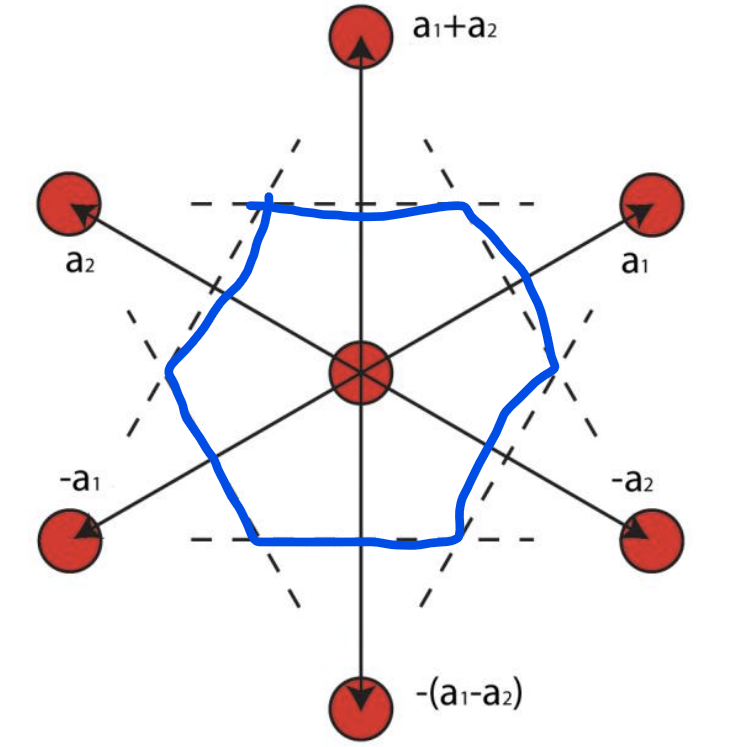
\includegraphics[width=\linewidth]{bilder_lf/heksagonalt_gitter_vektorer.png}
        \caption{Hekagonalt Gitterstruktur}
        \label{fig:heksagonalt_gitter_vektorer}
    \end{minipage}
    \hspace{0.5cm}
    \begin{minipage}[b]{0.45\linewidth}
        \centering
        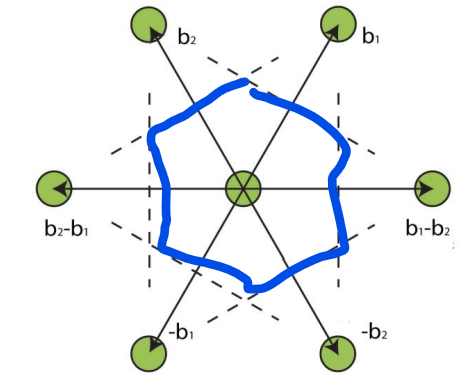
\includegraphics[width=\linewidth]{bilder_lf/resiprokalt_gitter_heksagonalt.png}
        \caption{Resiprokalt Heksigonalt Gitter}
        \label{fig:resiprokalt_gitter_heksagonalt}
    \end{minipage}
\end{figure}
\oppgave{3}
Den primitive cellen for F.C.C-strukturen vil se slik ut;
\begin{figure}
    \centering
    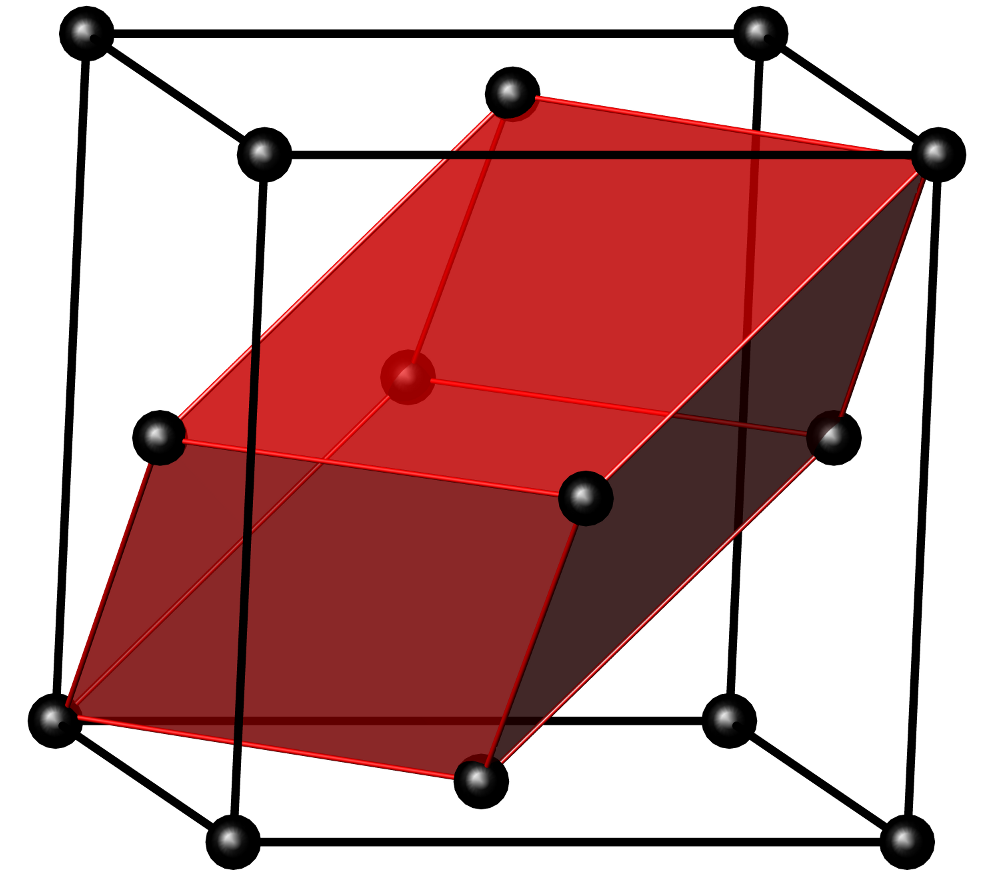
\includegraphics[width=0.5\linewidth]{bilder_lf/primitiv_struktur_fcc.png}
    \caption{Primitiv Enhetscelle F.C.C}
    \label{fig:primitiv_struktur_fcc }
\end{figure}
Her er vektorene svært lett å finne ut av. Spesielt hvis man velger origo nederst til venstre.
\nyside
\oving{3}
\oppgave{1}
\deloppgave{a}
La oss tegne et scenario på overflaten av en krystall:
\begin{figure}[H]
    \centering
    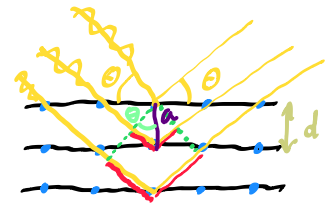
\includegraphics[width=0.5\linewidth]{bilder_lf/braggs_lov.png}
    \caption{Braggs Lov}
    \label{fig:braggs_lov}
\end{figure}

Hvis vi ser på denne figuren vil vi kunne få bølger som reflekteres på atomene inne i krystallen. For at de utgående bølgene på høyre siden skal interferere konstruktiv, må tilfellet være slik at de røde delene hvor bølgene har bevegd seg lengre inn i krystallen har bevegd seg på den første $\lambda$, i den andre $2\lambda$ og i den $n$-te $n \lambda$ lengre. Disse lengdene kan regnes ut i fra spredningsvinkelen og man vil få at:
\begin{equation}
    n \lambda = 2a \sin(\theta)
\end{equation}
Trigonometrien bak høyresiden kommer av at man må ha 2 ganger den ene siden av ren røde linjen. Denne røde linjen kan raskt regnes ut ved hjelp av de tegnede lengdene og vinklene.

Hovedantagelsen bak Braggs lov er at de atomiske lagene kan bli sett på som speil hvor inngangs- og utgangsvinklene er like. Videre antar vi at en del av bølgene er reflektert mens resten fortsetter til de neste lagene.
\deloppgave{b}
Kravene for å få diffraksjonsstråling er at bølgelengden til den innkommende strålingen må være sammenlignbart med atomavstanden og at Bragg-betingelsen  vi fant over er oppfylt. Den fysiske mekanismen bak diffraksjon er den samme som for spredning, men for historiske grunner er diffraksjonsbegrepet reservert for de sterktoppede interferensemønsterene som fremkommer i tilfellet med mange identiske spredere på et regulært gitter.

I tillegg til diffraksjonsbetingelsen beskrevet over, så må strukturfaktoren også selvfølgelig ikke være null.
\deloppgave{c}
Hovedbudskapet mellom Laue og Braggbetingelsene er matematisk identiske. Sagt raskt og ikke helt nøyaktig beskriver Lauebetingelsen hvordan konstruktiv interferense i resiprokalrommet ($\vec{Q}$ og $\vec{G}$), mens Braggs lov gir oss betingelsen for dette i det reelle rommet gjennom $\lambda$ og $a$. Braggs lov antar implisitt at vi har speilrefleksjon på gitterplanene, mens i $\vec{G} = \vec{Q}$ derivasjonen vil den fysiske meningen til disse planane fawlle ut av de mattematiske derivasjonene. Enda viktigere gir den fulle derivasjonen av $\vec{Q} = \vec{G}$ også et verktøy for å regne ut intensiteten til forskjellige diffraksjonstopper. Altså strukturfaktorer.
\deloppgave{d}
De tre mest brukte typene elektromagnetisk stråling er elektroner, røntgenstråler og nøytroner, med energier og bølgelengder som følger:
\begin{align}
    \text{Røntgen: }& E = \frac{hc}{\lambda}, \text{CuK}_{\alpha} \text{ stråling}; E \propto 8 \text{keV}, \lambda \propto 1.5Å \\
    \text{Elektroner: }& E = \frac{\hbar^2k^2}{2m}, k=\frac{2\pi}{\lambda}, \lambda = \frac{h}{\sqrt{2m_e}}, E \propto 100 \text{keV}, \lambda \propto 0.0004Å \\
    \text{Nøytroner(termiske): }& E = \frac{3}{2} k_B T \propto 25 \text{meV}, \lambda \propto 1.8Å
\end{align}
\oppgave{2}
Her er Cellene man kan få:
\begin{figure}[H]
    \centering
    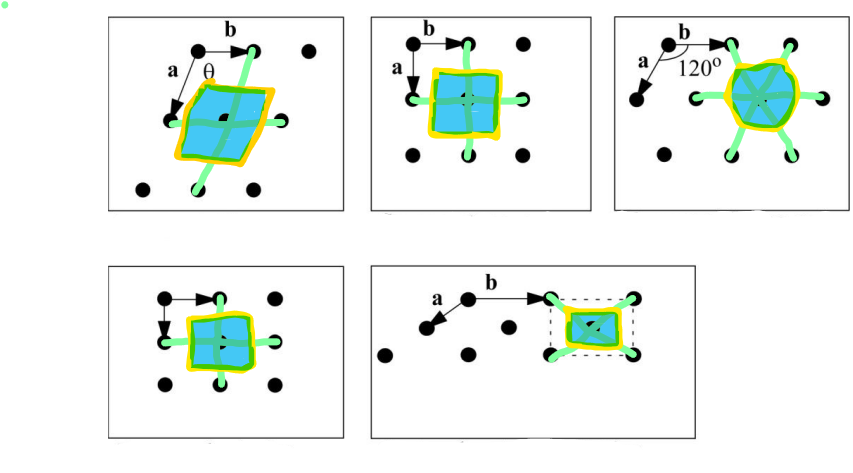
\includegraphics[width=0.85\linewidth]{bilder_lf/wigner_seitz_celler.png}
    \caption{Wigner Seitz-Celler}
    \label{fig:wigner_seitz_celler}
\end{figure}
\oppgave{3}
\deloppgave{a}
For å gjøre dette, skaper vi en Wigner-Seitz celle og velger et hjørne som origo som vi setter på et av atomene i gitteret. Dette kan da flyttes overalt for å ta med alle atomene og for å skape gitteret.

For F.C.C gitteret får vi de primitive enhetsvektorene:
\begin{equation}
    \vec{a}_1 = \frac{a}{2}(0, 1, 1) \tab[1cm] \vec{a}_2 = \frac{a}{2}(1,0,1) \tab[1cm] \vec{a}_3 = \frac{a}{2}(1,1,0)
\end{equation}
Man ser raskt at alle disse har lengde $a \frac{\sqrt{2}}{2}$, og vinkelen mellom dem blir 60 grader. Denne enhetscellen inneholder 4 Bravaisgitterpunkter. Volumet kan også bli regnet ut raskt ved hjelp av de tre vektorene og blir til $a^3 / 4$.

For B.C.C gitteret får vi de primitive enhetsvektorene:
\begin{equation}
    \vec{a}_1 = \frac{a}{2}(-1, 1, 1) \tab[1cm] \vec{a}_2 = \frac{a}{2}(1,-1,1) \tab[1cm] \vec{a}_3 = \frac{a}{2}(1,1,-1)
\end{equation}
Med disse får vi vinklene mellom dem som er $\arccos(-1 / 3) \approx 109.4 \text{deg}$, en lengde på $a \frac{\sqrt{3}}{2}$ og et volum på $a^3 / 2$.
\deloppgave{b}
Den minste verdien til høyden til basisen, blir slik at sfærene i det øvre laget akkurat treffer tre atomer under. Da vil sfærene i det nedre laget og en sfære i det øvre laget skape et tetrahedron. Så spørsmålet blir da, hva er høyden til dette tetrahedronet. Vel, vi kan finne det fra å forestille oss høyden som en trekant. Avstanden til midten her, vil bli midten av tre sfærer som treffer hverandre. Altså må midten bli til midten av en trekant med sidekanter d og vinkler som er 60 grader. For å finne lengden inn, får vi da at $d = a\tan(30 deg)$. Dette er da fra midten av kantene til trekanten. Ikke der atomene sitter. Nå får vi videre at høyden opp må bli nøyaktig slik at lengden ned til hjørnene blir til $2d$. Altså må:
\begin{align}
    d^2 + y^2 &= 4a^2\\
    \Rightarrow y^2 &= 4a^2 - d^2\\
    &= 4 - \tan(30 deg)^2 \\
    &= 4 - \frac{4}{3}
    &= \frac{8}{3}
    \Rightarrow y &= \sqrt{\frac{8}{3}}
\end{align}
Pakkefaktoren blir da volumet til 2 sfærer totalt delt på volumet til cellen vi ser på. Volumet til cellen vi ser på blir da en forskyvet kube på grunn av sfæreorientasjonen. Vinkelen eksisterer bare oppover og er da $\alpha_3$ og kan raskt regnes ut. Vi får at:
\begin{equation}
    \phi = \frac{2 \frac{4}{3} \pi \left(\frac{a}{2}\right)^3}{c a^2 \sin(\alpha_3)} = \frac{\pi}{3 \sqrt{2}} \approx 0.7405
\end{equation}
Dette er nøyaktig samme pakkefraksjon som for F.C.C gitteret. Altså er pakkefraksjonen likt for F.C.C som for H.C.P.
\oppgave{4}
En resiprokalgittervektor er definert av at $e^{iGR} = 1$. Her ville vi fått:
\begin{align}
    e^{iG_1 R} = e^{iG_2 R} e^{i G_3 R} = 1 * 1 = 1
\end{align}
Man kan også bruke at:
\begin{align}
    G_1 &= G_2 + G_3 =(h_2 b_1 + k_2 b_2 + l_2 b_3) + (h_3 b_1 + k_3 b_2 + l_3 b_3) \\
    &= (h_2 + h_3) b_1 + (k_2 + k_3) b_2 + (l_2 + l_3) b_3
    &= h_1 b_1 + k_1 b_2 + l_1 b_3
\end{align}
Altså blir $G_1$ bare en ny gittervektor.
\oppgave{5}
\deloppgave{a}
Atomformfaktoren $f(\vec{Q})$ er definert som Fourier-transformasjonen av elektrontettheten $\rho_c(\vec{r})$ slik som:
\begin{equation}
    f(\vec{Q}) = \int \rho_c(\vec{r}) e^{-i \vec{Q} \cdot \vec{r}} dV
\end{equation}
\deloppgave{b}
Her må vi enkelthen løse et integral:
\begin{align}
       f(\vec{Q}) &= \int \rho_c(\vec{r}) e^{-i \vec{Q} \cdot \vec{r}} dV \\
       &= \int_0^{2\pi} d \phi \int^{1}_{-1} \int^{\infty}_0 r^2 dr d(\sin(\theta)) e^{i \vec{Q} \cdot \vec{r}} \frac{1}{\pi a_0^3} e^{-2r / a_0}\\
       &= \frac{2}{ a_0^3} \int^{1}_{-1} \int^{\infty}_0 r^2 dr d(\sin(\theta)) e^{i Qr \sin(\theta)} e^{-2r / a_0}\\
       &= \frac{2}{ a_0^3}\int^{1}_{-1} \int^{\infty}_0 r^2 dr \frac{1}{i Q r} (e^{i Qr} - e^{-i Qr}) e^{-2r / a_0} \\
       &= \frac{4}{ a_0^3 Q} \int^{\infty}_0 r dr \sin(Qr) e^{-2r / a_0} \\
       &= \frac{4}{ a_0^3 Q} \int^{\infty}_0  dr r \sin(Qr) e^{-2r / a_0}  \\
        &= \frac{16}{(4 + Q^2 a_0^2)^2}\eqexplain{Her brukte vi det gitte integralet.}
\end{align}
\nyside
\oving{4}
\oppgave{0}
\deloppgave{a}
Her kan vektorene A og B spenne planet. Disse er definert som:
\begin{align}
    \vec{A} = -u \vec{a}_1 + v\vec{a_2}\\
    \vec{B} = -u \vec{a}_1 + w\vec{a_3}
\end{align}
Normalvektoren til dette planet er kryssproduktet til disse vektorene. Dette blir som følger:
\begin{align}
    \vec{A} \times \vec{B} = uvw( \frac{1}{u} \vec{a}_1+\frac{1}{v} \vec{a}_2+\frac{1}{w} \vec{a}_3)
\end{align}
Inversen av disse lengdene er jo $hkl$ lengdene våre multiplisert med en konstant. Altså har vi at:
\begin{align}
    \vec{A} \times \vec{B} &= uvw( \frac{1}{u} \vec{a}_1+\frac{1}{v} \vec{a}_2+\frac{1}{w} \vec{a}_3) \\
    &= uvw( Kh \vec{a}_1+Kk \vec{a}_2+Kl \vec{a}_3)\\
    &= uvw K\underbrace{( h \vec{a}_1+k \vec{a}_2+l \vec{a}_3)}
\end{align}
Og dermed ser vi at vektoren som har parantes under seg. Denne vektoren er jo vektoren i retningen (hkl). Altså må planet i seg selv være ortogonalt med denne vektoren siden planets normalvektor er parallelt med den retningen.

Vi vil vise at $d_{hkl} = \frac{2\pi}{|\vec{G}_{hkl}|}$. Måten vi gjør det er ved å starte å se på normalvektoren til et av planene våre. Den normaliserte normalvektoren vår i dette tilfellet blir:
\begin{equation}
    \vec{n}= \frac{ \vec{A} \times \vec{B}}{| \vec{A} \times \vec{B}|} = \frac{1}{a} \frac{( h \vec{a}_1+k \vec{a}_2+l \vec{a}_3)}{\sqrt{h^2 + k^2 + l^2}}
\end{equation}
Planene vil bli en forskyvning langs aksene med en lengde 1. Altså vil vi finne lengden mellom planene til å være en translasjon langs en av aksene prosjektert på  normalvektoren. Da vil få få:
\begin{align}
    d_{hkl} &= \frac{\vec{a}_i \cdot \vec{n}}{(h, k, l)} \\
    &= \frac{1}{(h, k, l)} \frac{(h, k, l) |\vec{a}_i|^2}{a \sqrt{h^2 + k^2 + l^2}} \\
    &= \frac{a^2}{a\sqrt{h^2 + k^2 + l^2}} \\
    &= \frac{a}{\sqrt{h^2 + k^2 + l^2}} \\
    &= \frac{2 \pi}{|\vec{G}_{hkl}|}
\end{align}
Dette fordi:
\begin{equation}
     |\vec{G}_{hkl}| = \frac{ 2 \pi \sqrt{h^2 + k^2 + l^2}}{a}
\end{equation}

\begin{figure}[h]
\begin{minipage}{0.55\textwidth}
Oppsummert er prosessen vi bruker for å finne denne lengden:
\begin{itemize}
\item Vi finner normalvektoren til planene. Som tegnet rosa i figuren til høyre.
\item Vi forskyver normalvektoren langs en av gittervektorene. Som langs den blå pilen til høyre.
\item Deretter finner vi lengden til projeksjonen av den blå vektoren (gittervektoren) langs den rosa vektoren (normalvektoren). Dette vil da gi oss gitterplanavstanden.
\end{itemize}
Altså kan dette illustreres velidg lett slev om det virkel ganske så komplisert. Den eneste forskjellen for resiprokalgitteret i motsetning til figuren er at man tar $2 \pi$ delt på inversen av lengden til resiprokalgittervektoren for å finne lengden i det reelle rom.
\end{minipage}
\begin{minipage}{0.4\textwidth}
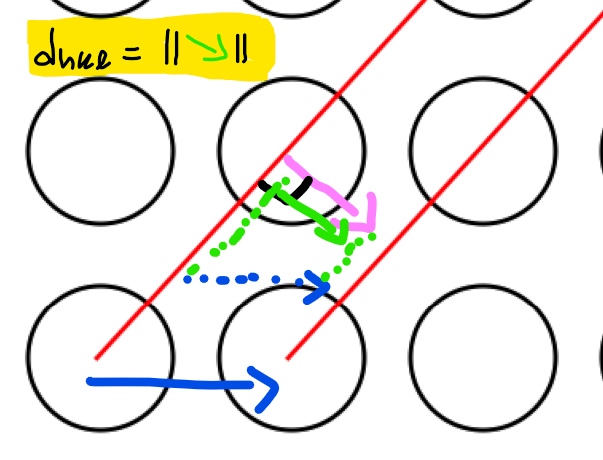
\includegraphics[width=\textwidth]{bilder_lf/illustrasjon_av_gitteravstander.png}
\caption{Illustrasjon av gitteravstander}
\label{fig:illustrasjon_av_gitteravstander}
\end{minipage}
\end{figure}
\deloppgave{b}
Som vist i starten av oppgave a) vil gittervektorene være vinkelrette på planet. Siden resiprokalgittervektorene er parallelle med gittervektorene må de også være vinkelrette på planet.
\deloppgave{c}
Utdødde refleksjoner oppstår når det er tilleggsegenskaper i den primitive enhetscella (vanligvis sentrerte atomer som i BCC- og FCC-strukturene) som skaper destruktiv interferens. Dette selv om hkl gitterplanene skulle gi opphav til diffrakterte stråler i henhold til Braggs lov.
\oppgave{1}
\deloppgave{a}
Den sammenhengende energien spiller en nøkkelrolle i å forstå de fysiske og kjemiske egenskapene til faste stoffer. Den representerer den totale energien som kreves for å bryte alle de kjemiske bindingene som holder et fast stoff sammen og separere dets atomer til sine isolerte tilstander. I et ionisk krystall, som inneholder positive og negative ioner, består den sammenhengende energien av flere komponenter. Gitterenergien er den primære bidragsyteren og representerer den elektrostatiske tiltrekningen mellom de motsatte ladningene av ionene i krystallen. I tillegg må vi vurdere ioniseringsenergien, som er energien som kreves for å fjerne et elektron fra et atom og danne et positivt ion, samt elektronaffiniteten, som er energien frigjort når et atom aksepterer et elektron for å danne et negativt ion. Dermed kan den sammenhengende energien betraktes som en samlet indikator på den sterke interaksjonen mellom atomene i et fast stoff, og dens nøyaktige verdi kan ha betydelige implikasjoner for materialets egenskaper og reaktivitet.
\deloppgave{b}
Det første leddet er koblet til Fermis ekslusjonsprinsipp som holder fermioner ifra hverandre. Altså kreves det uendelig mye energi å sette sammen to fermioner. Det andre leddet derimot kommer av dipol-vekselvirkninger og kalles for Van-der-waal vekselvirkninger. Som tatt fra forelesningsnotatene:

\begin{quote}
    Her skaper $r^6$ en Van der Waals vekselvirkning. Også kjent som London-vekselvirkningeen eller den induserte dipol-dipol vekselvirkningen. Det er hoved-tiltrekningskraften i krystaller av ikke-reagerende gasserr og i krystaller av mange organiske molekyler. Vekselvirkningen er en kvanteeffekt siden konstanten her vil avhenge av $\hbar$ og vil dermed forsvinne når vi tar grensen $\hbar \rightarrow 0$. Den vil også avhenge av $\alpha$ som er den elektroniske polariserbarheten.

    Kraften oppstår som følge av en midlertidig endring i elektrontettheten. Spesifikt kan elektrontettheten midlertidig skifte til å være større på den ene siden av kjernen. Dette skiftet genererer en midlertidig ladning som et nærliggende atom kan bli tiltrukket av eller frastøtt av.
    
    Videre skaper $r^{12}$ faktoren, kreftene forårsaket av Pauli's utelukkelsesprinsipp. Dette prinsippet går ut på at to fermioner ikke kan overlappe helt. Altså kan de ikke ha helt like kvantetall. Dette er i motsetning til bosoner. På grunn av dette vil det skapes en effektiv kraft mellom elektroner som holder dem unna hverandre som vil ha et potensial i form av $\frac{A}{r^{12}}$.
\end{quote}
\deloppgave{c}

\begin{table}[h]
\centering
\begin{tabular}{ll}
\toprule
Type binding & Forklaring \\
\midrule
Ionisk & Elektrostatiske tiltrekninger mellom positive og negative ioner \\
Kovalent & Deling av elektroner mellom atomer for å oppnå stabilitet \\
Metallisk & Delokalisert elektronstrømning blant metallatomer \\
Van der Waals & Svake intermolekylære krefter mellom nøytrale molekyler på grunn av midlertidige \\ & polariseringsendringer i dipoler. \\
Hydrogen & Hydrogenbindinger mellom hydrogenatomer og elektronegative atomer \\
\bottomrule
\end{tabular}
\caption{Ulike bindingstyper i krystaller.}
\label{tab:bindingstyper}
\end{table}
\deloppgave{d}
Ewald-konstruksjonen er en nyttig visualisering av Laue-betingelsen $\vec{Q}=\vec{G}$. Krystallgitteret er vist ved de resiprokale gitterpunktene i svart. Retningene til den innkommende og reflekterte strålen vises av de to vektorene $\vec{k}$ og $\vec{k'}$. Endepunktet til k er plassert ved opprinnelsen til rekrystalliserende rom, og en sirkel (2D) eller kule (3D) er tegnet med senter ved startpunktet til $\vec{k'}$. Hvis sirkelen skjærer en annen rekrystallisert gitterpunkt, vil en diffraktert stråle bevege seg i retning av $\vec{k'}$.
\begin{figure}[H]
    \centering
    \includegraphics[width=0.5\linewidth]{bilder_lf/ewaldsfæren.png}
    \caption{Ewald Sfæren}
    \label{fig:ewaldsfæren}
\end{figure}
Dette er dermed en fin måte å se på hvordan diffraksjon foregår i det resiprokale gitteret i motsetning til i reelt rom.
\deloppgave{e}
Radiusen til Ewald-kula er gitt ved k = |k|. Det forstås fra figuren at ved å tilfeldig orientere krystallen, er sannsynligheten for å oppfylle diffraksjonsbetingelsen lav. For å systematisk finne Bragg-refleksjoner, kan man:
\begin{itemize}
    \item Endre bølgelengden (Laue-metoden)
    \item Endre orienteringen ved å rotere prøven
    \item Bruke en polykrystallinsk prøve (Debye-Scherrer-metoden). Dette vil da gi større sannsynlighet for å skape diffraksjon i en av de krystallinske strukturene.
\end{itemize}
\deloppgave{f}
For slike celler vil vi ikke lenger ha perfekte $\delta$-funksjoner men på en viss måte uskarpe delta-funksjoner. Da vil vi ikke lenger ha perfekte punkter for Ewald-sfæren å treffe, men regioner, som da vil øke sannsynligheten for diffraksjon betydelig, avhengig av hvor skarpe delta-funksjonene blir.

Det ytterste tilfellet av dette er når prøven bare er ett atom tykt i én eller flere dimensjoner, slik som for eksempel en ultratynn film (som effektivt er 2D). Fourier-transformasjonen av en Dirac-delta, som nå tilnærmer tykkelsen på filmen, er en konstant. Derfor blir Bragg-punktene i resiprokalrommet utvidet til uendelige linjer orientert parallelt med filmens normal. Dermed økes diffraksjonsmulighetene betydelig.

Vi ser derfor at nanoskala-informasjonen om prøvens form og størrelse er kodet inn i rekrystalliseringrommet (og dermed inn i spredningsmønsteret). Med andre ord kan diffraksjonsteknikker brukes (og brukes også!) for å trekke ut informasjon om nanostrukturer og -enheter.

\oppgave{2}
\begin{itemize}
    \item Basert på Ewald-sfæren i \ref{fig:ewaldsfæren}, kan vi raskt se at $|Q| = 2k \sin(\theta)$. Vi vet derimot også at for å få diffraksjon så må $|Q| = |G|$ hvor $G$ er en vektor mellom to resiprokalgitterpunkter. Altså en resiprokalgittervektor. Videre vet vi at disse vektorene er $n G_0$ hvor $G_0$ er den minste mulige gittervektoren, som da har lengde $|G_0| = 2 \pi / d$. Altså har vi: $ 2k \sin(\theta) = |Q| = |G| = n 2 \pi / d$. Til slutt blir da $k =2\pi / \lambda$. Som gir oss:
    \begin{align}
        \frac{4 \pi}{\lambda} \sin(\theta) &= \frac{2 n \pi}{d} \\
        \Rightarrow n \lambda = 2 d \sin(\theta)
    \end{align}
    \item Siden vi nå er utledet Braggs lov fra Laue-betingelsen må disse to være ekvivalente.
\end{itemize}
\oppgave{3}
\deloppgave{a}
Den viktigste meknaismen bak dette er elektrostatiske (Coulomb) krefter som er tiltrekkende.
\deloppgave{b}
\begin{align}
    \alpha &= 2 (1 - \frac{1}{2} + \frac{1}{3} + \dots) \\
    &= 2\ln(2)
\end{align}
\deloppgave{c}
I NaCl atomet finnes det tre typer næreste nabo:
\begin{enumerate}
    \item Vi har 8 hjørner med avstand $\sqrt{3}$ fra sentrum, med en åttenedels ladning hver.
    \item Vi har 4 * 4 = 12 sidekanter med avstand $\sqrt{2}$ fra sentrum med en fjerdedels ladning hver. Disse har motsatt ladning fra de andre.
    \item Vi har 6 atomer på sideplanene med avstand 1 fra sentrum, med en halv ladning hver.
\end{enumerate}
Da får vi at$\alpha = 8\cdot\frac{1}{8} \cdot\frac{1}{\sqrt{3}} + 
 (-1) \cdot 12 \cdot \frac{1}{4}\cdot \frac{1}{\sqrt{2}} + 6 \cdot \frac{1}{2} \cdot 1 \approx 1.456 $.
\oppgave{4}
\deloppgave{a}
I den typiske enhetscellen har F.C.C-gitteret, punkter på $(0,0,0), (0, 1/2, 1/2), (1/2, 1/2,0)$ og $(1/2, 0, 1/2)$. Dermed kan vi bruke formelen for strukturfaktoren:

\begin{align}
    S &= \sum_j f e^{-i 2 \pi(h x_j + k y_j + l z_j)} \\
    &= f\left(1 + e^{-i \pi (k + l)} + e^{-i \pi (h + k)} + e^{-i \pi (h+l)} \right)\\
    &= f\left(1 + (-1)^{(k + l)} +  (-1)^{(h + k)} + (-1)^{ (h+l)} \right)
\end{align}
Hvis alle indeksene er odde, vil vi bare få $ S =4f$. Når en eller to av indeksene er like vil vi få $S=0$.
\deloppgave{b}
Siden diamantgitteret kun er to overlagte F.C.C-gittere hvor den ene er forskyvet $(1/4, 1/4, 1/4)$ i forhold til den andre, får vi følgende punkter: $(0,0,0), (0, 1/2, 1/2), (1/2, 1/2,0), (1/2, 0, 1/2), (1/4, 1/4, 1/4), (1/4, 3/4,  3/4), ( 3/4, 3/4,1/4)$ og $ ( 3/4, 1/4,  3/4)$. Altså har vi:
\begin{align}
   S &= \sum_j f e^{-i 2 \pi(h x_j + k y_j + l z_j)}  \\
   &= f\underbrace{\left(1 + (-1)^{(k + l)} +  (-1)^{(h + k)} + (-1)^{ (h+l)} \right) }_{\text{F.C.C strukturfaktoren}}\cdot (1 + e^{-i \frac{\pi}{2} (h+k+l)})
\end{align}
Venstredelen som er spesiell for diamantstrukturen vil ikke være null hvis alle indeksene er odde eller like. Altså får vi samme diffraksjonsbetingelser som tidligere.

\deloppgave{c}
Vi kan se at strukturfaktoren blir produktet av to forskjellige deler. En del som er F.C.C og den andre delen som blir spesifikt for diamantgitteret. Måten man kan se på dette er at disse to faktorene er egentlig konvolusjonen av F.C.C-strukturen med en basis av to atomer. En på $(0,0,0)$ og en annen på $(1/4, 1/4, 1/4)$. Siden vi har tatt fourier-transformen vil konvolusjonen bli til et produkt, slik som vi har her.
\nyside
\oving{5}
\oppgave{1}
\deloppgave{a}
Kort svar: Et fonon er den elementære eksitasjonen (kvanteenheten) av vibrasjoner i et krystallgitter. Et fonon har både partikkel- og bølgeegenskaper. Det er et boson. Det er en kvasipartikkel, noe som betyr at det er en kollektiv eksitasjon, men består ikke av materie.

Langt svar: Behandlingen av gittervibrasjoner i Kittels lærebok begynner med en klassisk derivasjon av spredningsrelasjonene for 1D-modeller. Det kan vises (se f.eks. Ashcroft og Mermin, Solid State Physics) at en 1-dimensjonal-kjede av N atomer (med ett atom per primitiv celle) kan betraktes som N harmoniske oscilatorer, hver med energiegenverdier:
\begin{equation}
    E = \left(n + \frac{1}{2}\right)\hbar \omega(k)
\end{equation}
Her er både $n$ og $k$ kvantetall. (Vi vil argumentere senere for at $k$ faktisk er diskret på grunn av periodiske grensebetingelser). Spredningsrelasjonen $\omega(k)$ kan vises å være den samme som vi har derivert klassisk for krystallvibrasjonene. Krystallens vibrasjonstilstander er spesifisert av eksitasjonstallene $n$ for hver modus $k$. Den kvantemessige enheten for disse vibrasjonstilstandene er kalt et fonon og er et kvasi-partikkel, analogt med fotoner. Som bosoner følger fononer Bose-Einstein-statistikk, og mange fononer kan lagres i samme modus $n$,$k$.
\deloppgave{b}

I polare krystaller er det veksling mellom positive og negative ioner. 

I den optiske moden er de nærliggende positive og negative ionene ute av fase, og det etableres en tidsvarierende elektrisk polarisering/felt, som tillater kobling til eksterne elektromagnetiske felt. For denne moden vil energien ikke gå mot null når impulsen gjør det. Vi har sett på dispersasjonsrelasjonen i forelesning og man kan faktisk se at dette blir et topppunkt til energien.

I den akustiske moden er de nærliggende positive og negative ionene i fase, og det er ingen netto forskyvning av ladning. Den akustiske grenen har energi $\hbar \omega$ som går mot null når $k$ går mot null. Lavenergi-akustiske krystallvibrasjoner er lydbølger.
\deloppgave{c}
Gruppehastigheten er definert som $v_g = \frac{\partial \omega}{\partial k}$. Den beskriver bølgepakkenes utbredelseshastighet, som vanligvis består av en sum av bølger med et kontinuum av frekvenser. Matematisk kan en bølgepakke i 1D uttrykkes som:
\begin{equation}
    u(x,t) \propto \int dk A(k) e^{i(kx -\omega(k) t)}
\end{equation}
hvor $A(k)$ er amplituden for et gitt $k$. Som understreket av notasjonen, på grunn av dispersjon ($\omega = \omega(k)$), vil hver bølgekomponent bevege seg med sin egen fasehastighet, og bølgepakken vil dermed endre form etter hvert som den sprer seg.

I tilfelle av en ikke-spredene bølgepakke (hvor $\omega = \omega_0$ for alle $k$), vil formen på bølgepakken bli bevart mens den sprer seg.

Energi og signaler transporteres med gruppehastigheten. Når $v_g = 0$ er det ingen transport av energi. Dette er tilfellet for stående bølger, der bølgepakken ikke beveger seg, til tross for at fasehastighetene er ikke-null.

\oppgave{2}
\deloppgave{a}
Dette vil fint modellere diatomiske molekyler. Kreftene mellom disse atomene i seg selv vil være mye sterkere enn kreftene mellom molekylene. Derfor trenger vi to typer fjærkonstanter, slik som vi har i modellen. Her vil vi derimot måtte ha samme masse på begge atomene i de diatomiske molekylene. For å utvide modellen må vi tillate forskjellige masser og orienteringer av dem.
\deloppgave{b}
Vi starter ved å skrive opp kraftlikningene vi vil få her. Vi bruker da den gitte figuren og får:
\begin{align}
    m \frac{d^2 u_s}{dt^2} &= -10C(u_s - v_s) - C(u_s - v_{s-1}) = 11 C u_s + 10C v_s + C v_{s-1} \\
    m \frac{d^2 v_s}{dt^2} &= -C(v_s - u_{s+1}) - 10C(v_s - u_{s}) = 10 C u_s - 11 C v_s + C u_{s+1} \\
\end{align}
Vi gjetter da at vi har løsningene:
\begin{align}
    u_s &= u e^{iska} e^{-i \omega t} \\
    v_s &= v e^{iska} e^{-i \omega t} \\
\end{align}
Ved å sette disse inn i likningene over, får vi likningssettet:
\begin{align}
     -\omega^2 m u_s &= -11 C u_s + 10 C v_s + C e^{-ika} \\
     -\omega^2 m v_s &= 10 C u_s - 11 C v_s + C e^{ika} 
\end{align}
Som kan skrives om til:
\begin{align}
    u_s (11C - \omega^2m) - v_s(10C + C e^{-ika}) &= 0\\
    -u_s (10C + Ce^{ika}) + v_s (11C - \omega^2 m)&= 0
\end{align}
Som kan skrives i matriseform (her kan vi bare bytte ut $u_s \rightarrow u$ og $v_s \rightarrow v$ siden alt deler samme faktorer utenom dette):
\begin{equation}
    \twomatrix{11C - \omega^2m}{-(10C + C e^{-ika})}{- (10C + Ce^{ika})}{11C - \omega^2 m} \twovec{u}{v} = 0
\end{equation}
For å løse denne likningen finner vi determinanten til matrisen og setter den lik null. Da finner vi følgende løsning for $\omega^2$:
\begin{equation}
    \omega^2 = \frac{11C}{m} \left(1 \pm \sqrt{1 - \frac{40}{121} \sin^2\left(\frac{ka}{2}\right))}\right)
\end{equation}
En graftegning av denne relasjonen vil bli:
\begin{figure}[H]
    \centering
    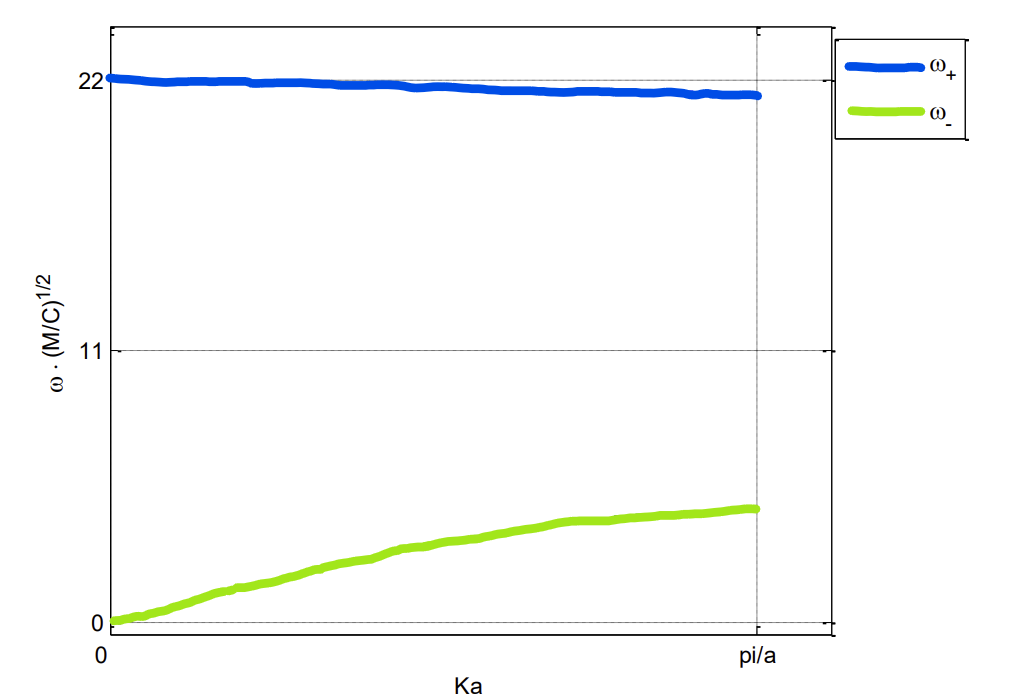
\includegraphics[width=0.75\linewidth]{bilder_lf/spredningsrelasjon_diatomisk_koblet.png}
    \caption{Negativ og positiv løsning av spredningsrelasjonen}
    \label{fig:spredningsrelasjon_diatomisk_koblet}
\end{figure}
\deloppgave{c}
Her kan vi ta likningssettet vi fant over bytte om $u$-er og $v$-er og få (når vi tar at $k \rightarrow 0$ som i oppgavebeskrivelsen):
\begin{align}
     -\omega^2 m u &= -11 C u + 10 C v + C \\
     -\omega^2 m v &= 10 C u - 11 C v + C
\end{align}
I det optiske tilfellet blir ikke $\omega = 0$ når $k \rightarrow 0$ og da kan vi dele likningene over på hverandre. Da får vi:
\begin{equation}
    \frac{u}{v} = \frac{-11 Cu + 11Cv}{11 Cu - 11 Cv} = -1
\end{equation}
I det akustiske tilfellet kan vi ikke gjøre dette. Da kan vi bruke en av likningene direkte. Vi bruker den øverste og får:
\begin{align}
    0 = -11 C u + 11 Cv\\
    \Rightarrow \frac{u}{v} = 1
\end{align}
Altså får vi at $\frac{u}{v} = \pm 1$ som er negativ i det optiske tilfellet og positivt i det akustiske tilfellet. Da ser vi at de to atomene vil vibrere sammen i det akustiske tilfellet og motsatt i det optiske tilfellet.
\oppgave{3}
\deloppgave{a}
I denne oppgaven tar vi simpelthen den deriverte av $U$ og setter utrykket lik null:
\begin{align}
    \frac{dU}{dr} &= 0 = -12 \frac{\sigma^12}{R^13} + 6\frac{\sigma^6}{R^7} \\
    \Rightarrow R &= \pm \sigma \sqrt[6]{2}
\end{align}
\deloppgave{b}
Situasjonen vi ser på kan bli tegnet slik:
\begin{figure}[H]
    \centering
    \includegraphics[width=0.75\linewidth]{bilder_lf/diatom_vanderwaal_ustødig.png}
    \caption{Vaklende atomstruktur i Leonard Jones}
    \label{fig:diatom_vanderwaal_ustødig}
\end{figure}
Her ser vi hvordan forskjellen i energi endrer seg. Vi har at endringen i energi blir den mørkegrønne energien minus den lysegrønne og den røde minus den lyserøde. Altså får vi:
\begin{equation}
    \Delta U = \underbrace{U(-u_{s-1} + a + u_s) - U(a)}_{\text{grønne delen}} +  \underbrace{U(a - u_s + u_{s+1}) - U(a)}_{\text{røde delen}}
\end{equation}
Dette kan vi videre Taylor-utvikle rundt a:
\begin{align}
     \Delta U &= U(-u_{s-1} + a + u_s) - U(a) +  U(a - u_s + u_{s+1}) - U(a) \\
     &= U(-u_{s-1} + a + u_s) +  U(a - u_s + u_{s+1}) - 2U(a) \\
     &\approx \frac{d U}{dR}\Bigg |_a (u_s - u_{s-1}) + \frac{d U}{dR}\Bigg |_a (u_{s+1}-u_s) + \frac{1}{2}\frac{d^2 U}{dR^2}\Bigg |_a (u_s - u_{s-1})^2 + \frac{1}{2}\frac{d^2 U}{dR^2}\Bigg |_a (u_{s+1}-u_s)^2
\end{align}
Her vil de to første leddene bli null av defininisjonen til $a$. Da får vi:
\begin{align}
    \Delta U &\approx \frac{1}{2}\frac{d^2 U}{dR^2}\Bigg |_a (u_s - u_{s-1})^2 + \frac{1}{2}\frac{d^2 U}{dR^2}\Bigg |_a (u_{s+1}-u_s)^2 \\
    &=\frac{36 \varepsilon}{\sqrt[3]{2} \sigma^2}\left((u_s - u_{s-1})^2 +(u_{s+1}-u_s)^2 \right)
\end{align}
Som helt klart viser oss det vi ville ha. Antagelsen vår her er jo da at $u_i$ er liten, så vi bare trenger å rekkeutvikle til andre orden. Videre antar vi at vi bare har to naboer til hvert atom. Egentlig gjelder jo alle, selv om de lengre unna gir et veldig lite bidrag.
\oppgave{4}
Vi kan tegne denne situasjonen slik:
\begin{figure}[H]
    \centering
    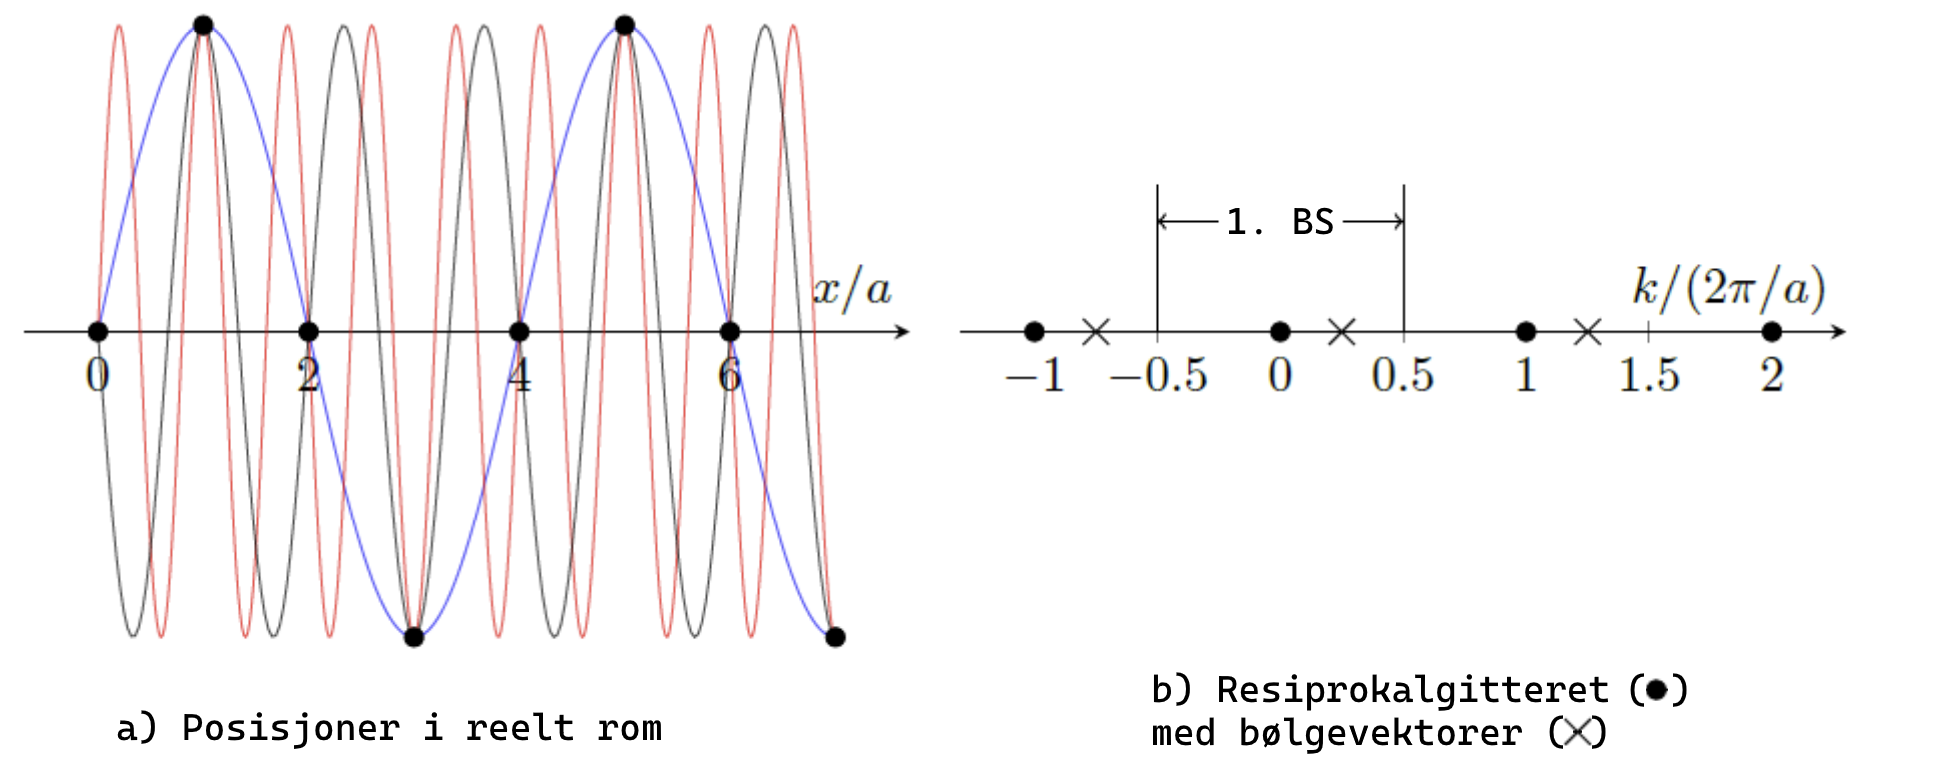
\includegraphics[width=0.55\linewidth]{bilder_lf/bølger_og_impulser_og_posisjon_øving_5.png}
    \caption{Bølger og resiprokalgittervektorer}
    \label{fig:bølger_og_impulser_og_posisjon_øving_5}
\end{figure}
\deloppgave{a}
Fordi bølgen bare er fysisk definert ved gitterpunktene, ser vi at hver av disse bølgefunksjonene beskriver bølgen like godt. Det er jo bare atomene som beveger seg i bølger på disse punktene. Med andre ord konkluderer vi med at alle disse $k$-verdiene beskriver den samme fysiske situasjonen. Følgelig må energien $\omega$ for disse tre modene også være den samme.
\deloppgave{b}
Figuren over (\ref{fig:bølger_og_impulser_og_posisjon_øving_5}) viser posisjonen til bølgevektorene $k$ i resiprokalrommet. Vi ser at alle $k$-verdiene er plassert like relativt til sine nærmeste resiprokale gitterpunkter, eller tilsvarende har de samme posisjonene innenfor sine respektive Brillouin-soner. All informasjon om vibrasjonsmodene finnes innenfor den første Brillouin-sonen!
\nyside
\oving{6}
\oppgave{1}
\deloppgave{a}
\begin{equation}
    \int d^3 \vec{r} \delta(\vec{r}) e^{.i \vec{k} \cdot \vec{r}} = e^{-i \vec{k} \cdot 0} = 1
\end{equation}
\deloppgave{b}
\begin{equation}
    \int d^3 \vec{r} \delta(\vec{r} - \vec{r}_0) e^{-i \vec{k} \cdot \vec{r}} = e^{- i \vec{k} \cdot \vec{r}_0}
\end{equation}
\deloppgave{c}
\begin{align}
    \int_0^\infty dx A e^{-a^2 x^2} e^{-ikx} &=  A \int_0^\infty dx e^{-a^2 x^2 -ikx} \\
   &=  A \int_0^\infty dx e^{-a^2 (x^2 -ikx / a^2)} \\
   &=  A \int_0^\infty dx e^{-a^2 (x + \frac{ikx}{2a})^2 + \frac{k^2}{4a^2}} \\
   &= Ae^{-\frac{k^2}{4a^2}} \frac{\sqrt{\pi}}{a}\\
   &= \frac{\sqrt{\pi} A}{a}e^{-\frac{k^2}{4a^2}} 
\end{align}
\deloppgave{d}
\begin{align}
    \mathcal{F}\{rect(x)\}(k) &= \int_{-a/2}^{a/2} e^{-ikx} dx \\
    &= \frac{e^{-iqa / 2 - e^{iqa/2}}}{iqa}\\
    &= a \text{sinc}\left(\frac{qa}{2}\right)
\end{align}
\deloppgave{e}
\begin{align}
      \mathcal{F}\{comb(x)\}(k) &= \int dx e^{-ikx} \sum^N_{n=1} \delta(x - na) \\
      &=\sum^N_{n=1} e^{-iqna}\\
      &=e^{-iqa} \frac{1- e^{-iqNa}}{1-e^{-iqa}}
\end{align}
Som kan bli skrevet om til:
\begin{equation}
    \mathcal{F}\{comb(x)\}(k) = e^{-iq(N-1)a/2}\frac{\sin(qNa/2}{\sin(qa/2)}
\end{equation}
Når $N$ går mot uendelig vil dette igjen bli til en uendelig sum av deltafunksjoner. Altså blir en uendelig kam i reelt rom til en uendelig kam i impulsrommet.
\oppgave{2}
Vi har her at:
\begin{align}
    n(\vec{r}) &= \sum_{\vec{q}}  n_{\vec{q}}  e^{i\vec{q} \cdot \vec{r}} \\
    &= n(\vec{r} + \vec{T})\\
    \Rightarrow& e^{i \vec{q} \cdot \vec{T}}\\
    \Rightarrow& \vec{q} \vec{T} = 2\pi n
\end{align}
Dette siste er den samme relasjonen som oppfylles hvis $\vec{G}$ er gittervektorer. Altså må $\vec{q} = \vec{G}$ og dermed har vi funnet det vi ville.
\oppgave{3}
\deloppgave{a}

Når man tar absoluttverdien av den komplekse Fourier-transformasjonen, blir argumentet (fasen) mistet, og man sitter igjen med amplituden til signalet. I diffraksjonsfysikk refereres dette til som faseproblemet. Fra et instrumentperspektiv er problemet at for å måle fasen til den innkommende bølgen, må detektoren måle det elektromagnetiske feltet ved optiske frekvenser (for synlig lys: ~$10^{15}$ Hz, for røntgen: ~$10^{18}$ Hz) – noe som for øyeblikket er svært vanskelig. Det var nettopp en ny rekord for å få til såpass høy deteksjon.

Bortsett fra: Legg merke til at i ultralydteknologi (som vanligvis brukes innen medisin), er frekvensen til (lyd)bølgen i 10 MHz-området, noe som kan måles elektronisk – derfor kan ultralyd danne bilder uten å bekymre seg for faseproblemet.

\deloppgave{b}
Hvordan i alle dager skal man finne ut av dette da?
\oppgave{4}
\deloppgave{a}
\begin{align}
    \mathcal{F}\{f(\vec{r}-\vec{r_0})\}(k) &= \int d^3 \vec{r} e^{i \vec{k}\cdot\vec{r}} f(\vec{r}-\vec{r_0})\\
        &= \int d^3 \vec{r} e^{i \vec{k}\cdot (\vec{r'}-\vec{r_0})} f(\vec{r'})\\
    &= e^{-i \vec{k}\cdot\vec{r_0}}\int d^3 \vec{r'} e^{i \vec{k}\cdot \vec{r'}} f(\vec{r'})\\
    &= e^{-i \vec{k}\cdot\vec{r_0}}\int d^3 \vec{r} e^{i \vec{k}\cdot \vec{r}} f(\vec{r})\\
    &= e^{-i \vec{k}\cdot\vec{r_0}} \mathcal{F}\{f(\vec{r})\}(k)
\end{align}
\deloppgave{b}
Fourier-transformen av krystallstrukturen vil da kreve en til fasefaktor som vist i teoremet over. Derimot avhenger formen av spredningsmønsteret kun av absoluttverdien til strukturfaktoren. Altså vil denne fasefaktoren kanselleres og vi står igjen med nøyaktig samme mønster. Altså ingen endring.
\oppgave{5}
Siden spredningsintensiteten vil avhenge av fourier-transformasjonen av elektrontettheten i annen vil vi her få fourier-transformasjonen av en konvolusjon av et gitter med todimensjonale rektangeler $Na \times Mb$. Dette blir til et produkt i fourierrommet og derfor får vi at $I \propto F^2 \propto(\mathcal{F}\{\text{gitter}\} \cdot \mathcal{F}\{\text{rektangel}\})$ som gjør at vi vil få noe proporsjonalt med  sinc-funksjonene vi fant tidligere, som var fourier-transformasjoner av rektangelene, multiplisert med deltafunksjoner. I realiteten med et endelig gitter blir disse ikke deltafunksjoner men blir glattet ut. Videre vil a-lengden bli lengst i impulsrommet siden det er kortest i det reelle rommet. Da kan vi tegne noe som:
\begin{figure}[H]
    \centering
    \includegraphics[width=0.5\linewidth]{bilder_lf/diffraksjon_av_rektangulært_gitter.png}
    \caption{Diffraksjon av gitter med rektangulære enhetsceller}
    \label{fig:diffraksjon_av_rektangulært_gitter}
\end{figure}
\nyside
\oving{7}
\oppgave{1}
\deloppgave{a}
Mattematisk gir varmekapasiteten deg muligheten til å finne ut av hvor vanskelig det er å varme opp et stoff. Hvor mye energi som krevet for å gjøre dette og hvor raskt det kan skje. Mattematisk er det definert som:
\begin{equation}
    \left(\frac{\partial U}{\partial T}\right)_{\text{V eller P konstant}}
\end{equation}
Grunnen til at vi ikke bryr oss om varmekapasiteten med endrene trykk er at arbeiden $dW = pdV$ vil være nær null og dermmed vil arbeidet gjort av en utvidene gass på omgivelsene være neglisjerbart. Altså har dette bidraget lite å si.
\deloppgave{b}
Forskjellen mellom disse partiklene er at bosoner har heltallsspinn mens fermioner ikke har dette. Dette gjør at man får paulis ekslusjonsprinsipp for fermionene så de ikke kan være i samme kvantetilstand. Faktisk vil de frastøte hverandre hvis man prøver dette. Med en uendelig kraft hvis de kommer uendelig nærme. Bosoner derimot liker å klumpe seg sammen og vil ha en tiltrekkende kraft mellom seg ved små avstander. Bosoner er for eksempel fononer og fotoner, mens fermioner er elektroner.
\deloppgave{c}
Planck-fordelingen beskriver antall bosontilstander i et gitt kvantenivå ved en viss temperatur. Mer nøyaktig er det sannsynligheten for okkupasjon ved en gitt temperatur. Fordelingen ser slik ut:
\begin{equation}
    <n(T)> = \frac{1}{e^{\beta \hbar \omega}-1}
\end{equation}
Gjennomsnittsantallet (forventningsverdien) av fononer i en gitt mode/kvantetilstand øker med temperaturen og avtar med energien til tilstanden $ E = \hbar \omega $. Dette kan tolkes slik at når temperaturen øker, vil det være flere fononer som okkuperer de ulike vibrasjonsmodusene, og dermed vil atomene i materialet vibrere mer kraftig. Hver mode er spesifisert ved sin gren (eller "polarisering") og bølgetall $k$.

Ved grensen for høy temperatur kan kvanteeffekter neglisjeres, og den klassiske Maxwell-Boltzmann-statistikken gir en god tilnærming til Planck-fordelingen. Med andre ord kan de diskrete energitilstandene og "frysing ut" av de høyere energimodusene ignoreres ved høye $T$, og ekvipartisjonsteoremet vil gjelde.

(En liten påminnelse: Planck-fordelingen er best kjent for å beskrive mengden elektromagnetisk stråling som sendes ut som funksjon av frekvens av en svart kropp i termisk likevekt.)
\deloppgave{d}
En stor del (nesten alt! hele 99\%) av den indre energien $U$ i faste stoffer kommer fra gittervibrasjonene. Okkupasjonen av fononer i de ulike tilstandene varierer med temperaturen. Ved å beregne den forventede fononokkupasjonen kan bidraget fra vibrasjonsenergien til den indre energien beregnes. Ved å differensiere energien $U(T)$ med hensyn til temperaturen, finner man fononenes bidrag til varmekapasiteten. Som er svært høy. Det andre bidraget kommer fra frie elektroner som  beveger seg rundt i stoffene. Også kalt ledningselektroner. Denne delen derimot svarer til kun 1\% av varmekapasiteten.
\oppgave{2}
\deloppgave{a}
Dette er fordi elektronene og atomene kun kan bevege seg i to dimensjoner. Altså vil ikke høyden eller den tredje dimensjonen ha noe å si. Altså vil det være helt likt om vi ser på det som to eller tredimensjonalt.

Mer presist er kriteriet for å neglisjere bevegelse normalt på planene at eksitasjonsenergien til fononer i modene som er normale på planene, $\hbar \omega$ er mye større enn den termiske energien $k_BT$. Dette sikrer at fonongrenene utenfor planet er i sine grunntilstander.
\deloppgave{b}
Her må vi bruke se på impulsrommet for å finne antall moder til en gitt energi. Vi har da at:
\begin{align}
    N &= \frac{\pi k^2}{\left(\frac{2\pi}{L}\right)^2}\\
      &= \frac{L^2}{4\pi} k^2\\
    \Rightarrow D_k(k) &= \frac{dN}{dk} = \frac{L^2}{2\pi}k\\
    \Rightarrow D_\omega(\omega) &= \frac{dN}{d\omega}\\
    &=  \frac{dN}{dk}(k(\omega))\frac{dk}{d\omega}\\
    &=  D_k(k(\omega))\frac{d(\frac{\omega}{v_g})}{d\omega}  \\
  &= D_k(k(\omega)) \frac{1}{v_g} \\
k(\omega) &= \frac{\omega}{v_g}\\
  \Rightarrow D_\omega(\omega)  &=\frac{L^2}{2\pi} \frac{\omega}{v_g} \frac{1}{v_g} \\
    &=\frac{L^2\omega}{2\pi v_g^2}
\end{align}
Her er jo da $v_g$ gruppehastigheten.
\deloppgave{c}
Vi har fra forelesning at:
\begin{equation}
     C_{\text{gitter}} = k_B \sum_p \int d\omega D_p(\omega) \frac{x^2e^x}{\left(e^x-1\right)^2} \tab[2cm] x = \beta \hbar \omega
\end{equation}
Her kan vi rett og slett sette inn fordelingsfunksjonen vår. Vi antar at polarisering ikke har noe å si. Da ser vi svært raskt at $d\omega$ være koblet til $T$ og det vil også $D(\omega)$ være. Dette på grunn av definisjonen vår til $x$. Siden disse er ganget sammen må da $C \propto T^2$. Skriver man ut hele utrykket ordentlig får man:
\begin{equation}
    C = \frac{dU}{dT} = \frac{d}{dT} \left(\frac{\hbar L^2}{\pi v_g^2} \frac{k_B^3 T^3}{\hbar^3}\right) \int \frac{x^2 }{e^x-1}
\end{equation}
En måte å faktisk finne $U$ er gjennom:
\begin{equation}
    U = \sum_p \int d\omega D_p(\omega) <n(\omega)> \hbar \omega
\end{equation}
Altså å summe over alle tilstander som finnes i hvert energinivå ganger energien på det nivået.
\deloppgave{d}
Med \underline{adjacent layers} mener man de lagene som er ved siden av hverandre. Da forventer vi igjen at man bare har et lineært gitt er. Siden $C_{3D} \propto T^3$ og  $C_{2D} \propto T^2$ vil en god antagelse være at $C_{1D} \propto T$. Dette holder derimot kun på ekstremt lave temperaturer
\oppgave{3}
\deloppgave{a}
For Debye-modellen er $\omega = v_g k$. I en dimensjon ghar vi da at (2eren fordi k kan være positiv og negativ):
\begin{align}
    N &= \frac{2|k|}{\left(\frac{2\pi}{L}\right)}\\
      &= \frac{L}{\pi} k\\
    \Rightarrow D_k(k) &= \frac{dN}{dk} = \frac{L}{\pi}\\
    \Rightarrow D_\omega(\omega) &= \frac{dN}{d\omega} \\
    &= \frac{dk}{d\omega}\frac{dN}{dk} \\
    &= \frac{1}{v_g}\frac{L}{\pi}
\end{align}
\deloppgave{b}
Nå kan vi gjøre:
\begin{align}
     D_\omega(\omega) &= \frac{dk}{d\omega} \frac{dN}{dk} \\
     &=\frac{L}{\pi } \frac{dk}{d\omega} \\
     &= \frac{L}{\pi } \frac{d}{d\omega} \frac{2}{a}\arcsin{\left(\frac{\omega}{2}\sqrt{\frac{M}{\gamma}}\right)}\\
     &= \frac{2L}{\pi a} \frac{d}{d\omega} \arcsin{\left(\frac{\omega}{2}\sqrt{\frac{M}{\gamma}}\right)}\\
     &= \frac{2L}{\pi a}  \frac{a}{\sqrt{4-\omega^2 \frac{M}{\gamma}}}\\
     &= \frac{2L}{\pi}  \frac{1}{\sqrt{4-\omega^2 \frac{M}{\gamma}}}
\end{align}
Tar vi at alle konstantene er like og plotter disse to sammen får vi:
\begin{figure}[H]
    \centering
    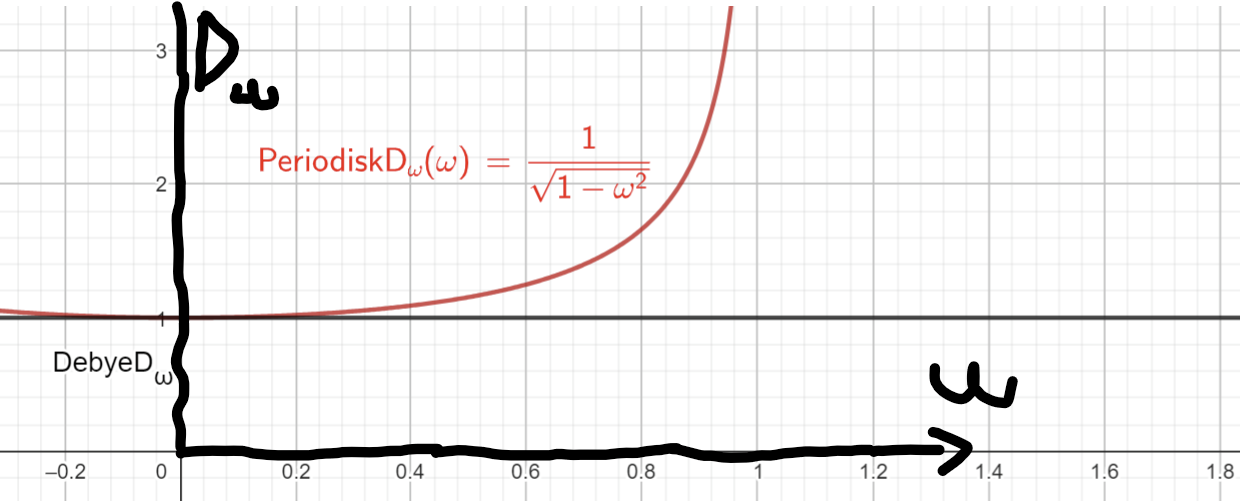
\includegraphics[width=0.4\linewidth]{bilder_lf/debye_versus_ekte_monoatomisk_kjede.png}
    \caption{Debye versus ekte monoatomisk kjede}
    \label{fig:debye_versus_ekte_monoatomisk_kjede}
\end{figure}
\nyside
\oving{8}
\nyside
\oving{9}
\nyside
\oving{10}
\nyside
\oving{11}
\newpage
\printbibliography
\end{document}